% !TeX encoding = UTF-8
% !TeX root = MAIN.tex

\chapter{Motivation}

The starting point of this thesis is recently conducted research that studies the link and possible causal effects between monetary policy decisions by the FED and the stock market in the U.S., not only in an ex-post but also in an ex-ante sense.

The paper Stock Returns over the FOMC Cycle \parencite{cieslak_stock_2019} finds a pattern in financial markets around the world that suggests that stock market excess returns in the last 23 were entirely earned in even weeks (0, 2, 4 and 6) starting from the last FOMC meeting. The authors tie their findings to a known phenomenon called "Fed Put", by which they mean accommodating monetary policy.

In a follow-up paper, The Economics of the FED Put \parencite{cieslak_economics_2021} the authors use textual analysis of FOMC (Federal Open Market Commitee) scripts to identify and measure the causal effect that policymakers indeed pay intention to the stock market, especially since the mid-1990s and stock market performance is linked with the FED’s internal growth projections. The authors further claim that even if the policymakers seem to be aware that a dynamic like the FED put could induce risk-taking behavior leading to moral-hazard implications, it does not particularly affect their decision-making in an ex-ante sense.

In my thesis, I aim to find out whether the financial pattern regarding stock excess returns in FOMC even weeks is still relevant from 2016 (which should not be the case, especially once the information has reached the market) onwards (probably complicated by the COVID-19 crisis) since the paper published in 2019 only investigates this pattern before 2016. Additionally, the authors prove the relevance of their financial pattern worldwide using exchange-traded funds (ETFs) containing European stocks. I want to include further results with a specific focus on European stock returns.

%In my thesis I aim to find out whether the "FED Put" remains relevant in the %Eurozone from 2016 onwards till 2023  and whether a similar dynamic can %be observed within the European Central Bank's policy, particularly concerning interest rates and Exchange-Traded Funds (ETFs) containing %European stocks. 

\chapter{What is the "FED Put" and how can it be explained?}
\section{The FED Put}
The FED Put in general refers to (or, moreover, to the expectation of) a strong accommodating monetary policy by the FED, by which, in case of a sharp decline in asset prices, the FED is expected by the market (its investors) to intervene. The term is coined from the concept of a "put option" in asset markets, which gives the buyer the option to sell at a predetermined price. Thus, the FED would protect an investor from the decline in the value of an asset.\footnote{\url{https://corporatefinanceinstitute. com/resources/economics/FED-Put/}}

Central banks have gained credibility ever since the mid-1980s by keeping inflation low \hyperref[item:hall_is_2011]{Hall (2011)} . The related term "Greenspan Put" is often used to describe the monetary policy under former Federal Reserve Chairman Alan Greenspan to intervene in financial markets in order to prevent significant declines or disruptions. 

While some argue that market interventions are necessary to prevent financial crises (like the Dot-com bubble burst in 2001 or Lehman Brothers in 2008), others believe that these interventions distort the market and create unnecessary moral hazard \hyperref[item:cieslak_economics_2021]{Cieslak and Vissing-Jorgensen (2021)},  meaning that investors are willing to take on excessive risks because they believe that the FED will always come to rescue them arguing that such "too big to fail” beliefs or mentality can lead to financial crises in the long run.

\section{Stock Returns over the FOMC Cycle}

Diving further into dynamics like the FED Put,  \hyperref[item:cieslak_stock_2019]{Cieslak et. al (2019)}, focuses on a FOMC cycle specific pattern of the equity premium since 1994. 
The stock returns exhibit a distinct,  statistically significant pattern over the FOMC cycle.  Notably,  it primarily accrues in even weeks of the FOMC cycle time (for a graphical explanation of the FOMC cycle, see figure~\ref{cies19_fig2} on page~\pageref{cies19_fig2}). For calculation of stock excess returns the authors use research portfolio data provided by Kenneth R. French for convenience\footnote{\url{https://mba.tuck.dartmouth.edu/pages/faculty/ken.french/data_library.html\#research}}.

\begin{figure}[h]
    \centering
    \label{cies19_fig1}
    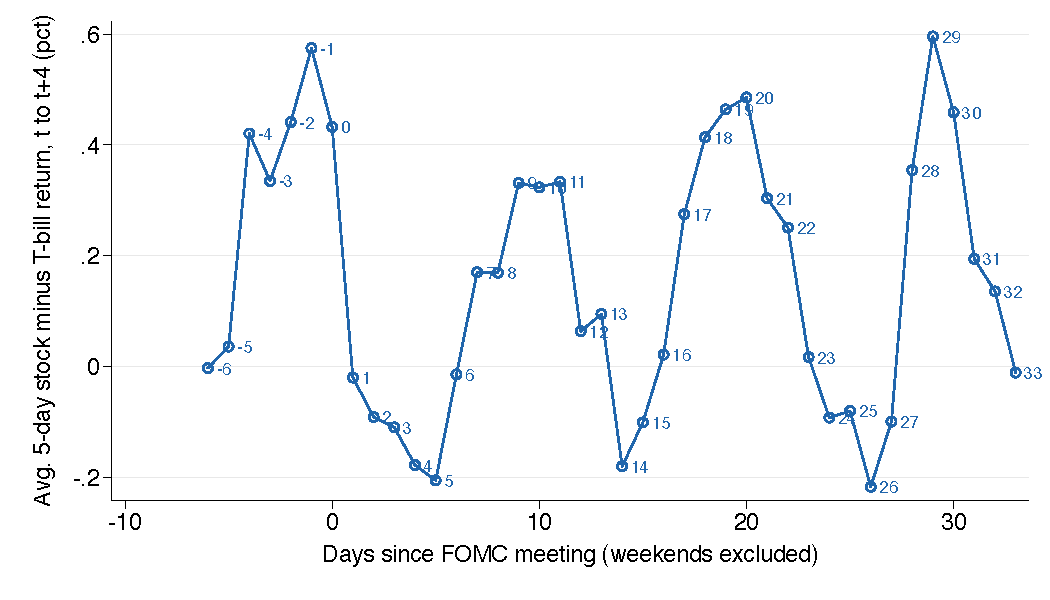
\includegraphics[width=0.9\textwidth]{figures/cies19/fig1}
    \caption{Average 5-day stock excess returns over FOMC cycle time (pct) \hyperref[item:cieslak_stock_2019]{(Cieslak et. al, 2019)} }
\end{figure}

The authors present three different trading strategies (A, B, and C) that demonstrate the influence of the FOMC cycle on stock market returns.  Of particular note is Strategy A, which involves exclusively holding stocks during even FOMC cycle weeks (and investing in a risk-free rate during odd FOMC cycle weeks). This strategy demonstrates that the average annual return more than doubles compared to holding for example an ETF throughout the entire FOMC cycle.  Conversly, the authors find that holding an ETF during uneven FOMC weeks (compared to a risk-free rate) resulted in financial losses over the examined period from 1994 to 2016.  This results have also been covered by the media.\footnote{\url{https://www.economist.com/finance-and-economics/2016/09/03/the-long-arm-of-the-FED}}

\begin{figure}[h]
    \centering
     \label{FED_long_arm}
    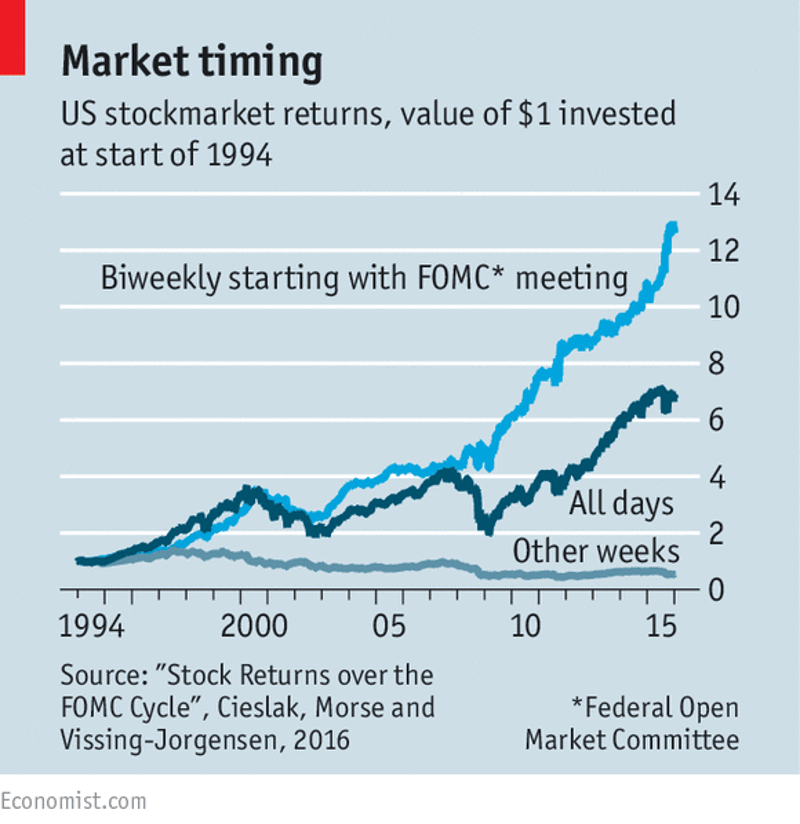
\includegraphics[width=0.6\textwidth]{figures/20160903_FNC453.png}
    \caption{"The long arm of the FED", \hyperref[item:noauthor_long_2016]{\textit{TheEconomist} (2016)}}
\end{figure}

The authors extend their analysis to explore whether the FOMC cycle return pattern extends beyond the United States, potentially influenced by movements of the dollar currency. To investigate this, they use ETFs containing globally diversified stocks. To establish causality, the authors compare FOMC cycles with other macroeconomic news calendars (e.g., Bloomberg macroeconomic news), dispelling the notion that macroeconomic news significantly correlates with FOMC cycle calendars. They also provide evidence that the release of quarterly firm profits does not substantially account for the observed equity premium patterns over the FOMC cycle.

The authors examine a causal link between the FED's policy actions and the behavior of the stock market by analyzing in the Federal Fund target changes between meetings,  FED funds futures and internal meetings of the Board of Governors. They propose that the FED's anticipated accommodative policies have a substantial impact on the stock market, resulting in a increase of the overall equity premium.  Additionally, they contend that there is evidence of informal communication channels between FED officials, the media, and the financial sector, which serve as a means for disseminating information about monetary policy to the market.

\begin{figure}[h]
    \centering
    \label{cies19_fig3A}
    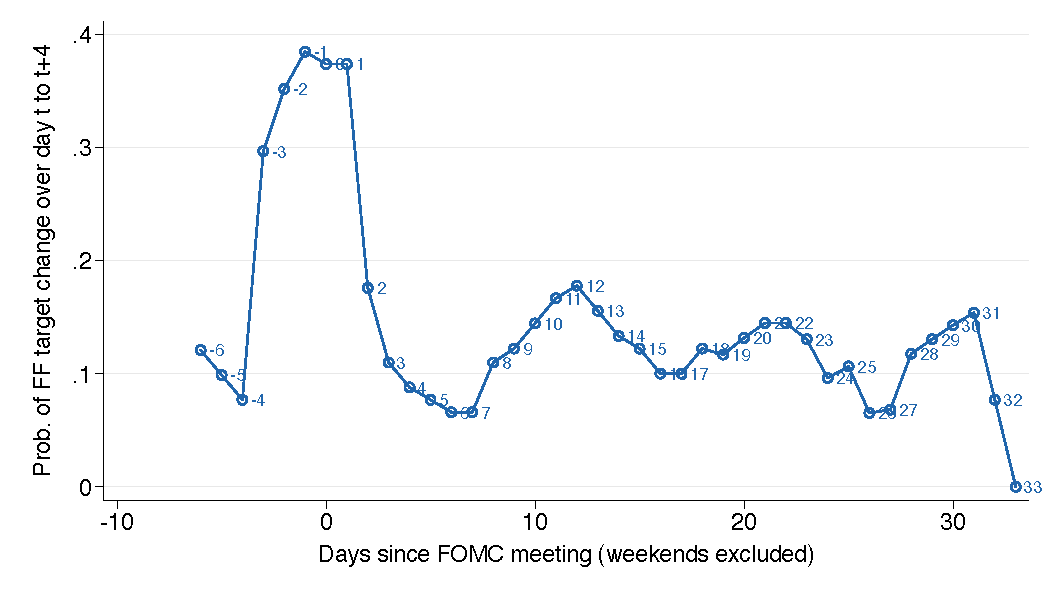
\includegraphics[width=0.9\textwidth]{figures/cies19/fig3A}
    \caption{Probability of FFR target changes within FOMC cycle time  \hyperref[item:cieslak_stock_2019]{(Cieslak et. al, 2019)}}
\end{figure}

\pagebreak

\section{The Economics of the FED Put}
\hyperref[item:cieslak_economics_2021]{Cieslak and Vissing-Jorgensen (2021)} further attempts to study the economics of the relationship between FED policy and the stock market. The authors compare the stock market's predictive power to other economic indicators to forecast changes in the Federal Funds Rate (FFR) using textual analysis from former FOMC meeting transcripts.\footnote{\url{https://www.federalreserve.gov/monetarypolicy/fomc_historical.htm}} Their findings affirm that the FED indeed pays a lot of attention to the stock market during market downturns.

\begin{figure}[h]
    \centering
        \label{cies21_fig5}
    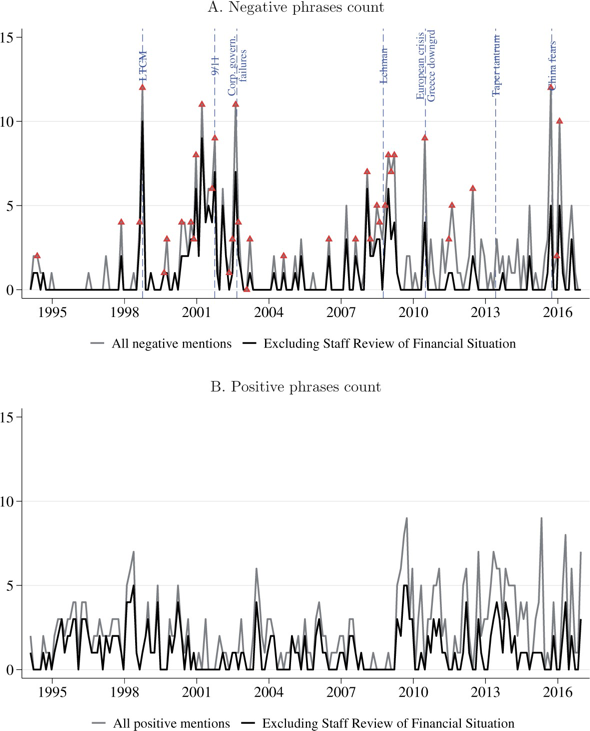
\includegraphics[width=0.9\textwidth]{figures/cies21/Figure5}
    \caption{Negative and positive phrases of the stock market count \hyperref[item:cieslak_economics_2021]{(Cieslak and Vissing-Jorgensen,  2021)}}
\end{figure}

They argue that the FED Put is fueled by the Federal Reserve's concerns about wealth effects on consumption. Conversely, strong stock market performance corresponds to updates of the FED’s internal growth projections. Empirical evidence substantiates their claims, as multiple regressions of changes in the FFR demonstrate that the stock market explains a higher proportion of the variance (R-squared) compared to other macroeconomic indicators. Importantly, this relationship appears to be less pronounced before the 1990s period.  

During the third European Central Bank (ECB) annual research conference \hyperref[item:european_central_bank_third_2018]{ (European Central Bank,  2018)}, valuable comments on the econometric approach by the authors were made by the discussant, Emmanuel Moench, the former head of research at the Bundesbank. Moench suggests that the correlation between stock excess returns and the FFR is heavily influenced by two specific FOMC meetings (during financial crises like the dot-com bubble burst in 2001 and the 2008 financial crisis). Furthermore, he recommended incorporating additional covariates, including consumer confidence news and credit spreads, into the regression models to enhance their explanatory power. Moench sees the stock market as one of several co-factors influencing Federal Reserve policy (presumably over the updates of the FED's growth projections as stated by the authors), rather than a dominant driver of the FED's policy.



\chapter{Stock returns over the FOMC Cycle Revisited }


\section{The FOMC cycle}

The FOMC meets approximately every eight weeks during the year,  resulting in an FOMC cycle time of approximately 7 weeks (excluding weekends) most of the time since a year has 52 weeks. The authors, therefore, define FOMC cycle time week dummy variables for week 0 as days -1 to 3, week 1 as days 4 to 8, and week 6 as days 29 to 33. Worth mentioning is that the authors drop 3 days, which would be in FOMC cycle week 7 from their investigation, and that the number of available data points decreases for FOMC dummies (meaning 920 days in week 0,  924 days in week 2,  831 days in week 4,  120 days in week 6 for the relevant timespan from 1994 to 2016).

\label{cies19_fig2}
\begin{figure}[h]
    \centering
    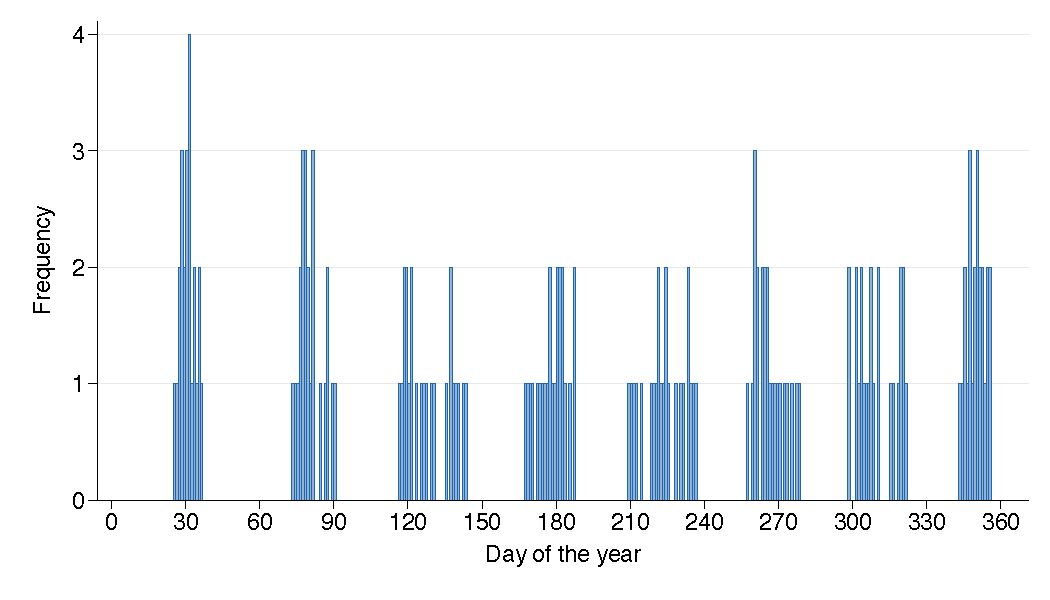
\includegraphics[width=0.75\textwidth]{figures/cies19/fig2}
    \caption{Frequency of FOMC meetings during the year from 1994 to 2016 \parencite{cieslak_stock_2019}}
\end{figure}


\section{Institutional Setting}

 The Federal Reserve System consists of the Board of Governors, 12 Federal Reserve Banks, and the FOMC. The 12 members of the FOMC implement monetary policy with the aim of achieving macroeconomic objectives, including adjusting federal fund rates and large-scale purchases of treasury securities and securities that were issued or guaranteed by federal agencies as policy instruments since the 2008 financial crisis (to lower long-term interest rates) to ensure the efficient functioning of the U.S. economy\footnote{\url{https://www.federalreserve.gov/aboutthefed.htm}}.  

\section{FOMC Data}

The FOMC publishes detailed records of its meeting proceedings on the Federal Reserve's webpage\footnote{\url{https://www.federalreserve.gov/monetarypolicy/fomccalendars.htm}}.  
Since the 1994 meetings,  the FOMC Secretariat has produced transcripts shortly after each meeting. 
The meeting participants have the opportunity to review the transcripts for accuracy within the subsequent weeks. .
These transcripts are available on the Federal Reserves webpage and contain a very small amount of confidential information that may be deleted. 
The FOMC schedules eight meetings annually,  issuing a policy statement after each meeting,  summarizing the economic outlook and their policy decisions. 
The Chairman holds press briefings to discuss policy decisions and economic projections. 
Meeting minutes are published three weeks after each regular meeting and complete transcripts are made available up to five years after the meeting.

\section{Measurement and estimation analysis (MEA)}

\subsection{MLR model}

One relevant multiple linear regression (MLR) model with dummy variables for even FOMC cycle weeks as in \parencite{cieslak_stock_2019} can be defined as:
\begin{equation}
	ex1_{i}=\beta_{0}+D_0*\gamma_{1}+D_1*\gamma_{2}+\epsilon_i
\end{equation}
where
\begin{equation}
    D_0=
    \begin{cases}
      1, & \text{If in week 0 of FOMC cycle time}\\
      0, & \text{Otherwise}
    \end{cases}
\end{equation}
is a function equal to 1 if the FOMC cycle dummy is in week 0,
\begin{equation}
    D_1=
    \begin{cases}
      1, & \text{If in week 2,4 or 6 of FOMC cycle time. } \\
      0, & \text{Otherwise}
    \end{cases}
\end{equation}
is a function equal to 1 if the FOMC cycle dummy is in week 2,  4 or 6,
$ {ex1_{i}} $ are the 1-day risk-free excess returns on stocks,
$ { \hat{\beta_{0}} } $ is the OLS-estimated intercept,
$ { \hat{\gamma_{1}}, \hat{\gamma_{2}} } $   and
$ { \epsilon_i \; \sim \; i.i.d.  \; \mathcal{N}\left(0, \sigma^2 \right) } $
are independent identically distributed OLS-estimated standard errors. 
The OLS-estimated parameters $ {\hat{\gamma_{1}}} $ is of more importance with subject to to the probability of intermeeting target changes (see figure ~\ref{cies19_fig3A}})

\subsection{FOMC dummies}

The R Code in \texttt{generate\_fomc\_dummies\_cycle\_dummies.R} (see Appendix)
generates FOMC week dummy variables by using the \texttt{"FOMC\_Cycle\_dates\_1994\_nov2023.xlsx"} file containing FOMC meeting dates for later estimation of the influence of the FOMC cycle on excess stock returns.

\subsection{Data Preprocessing}

The analysis commences with the importation and organization of two datasets. 
The first dataset, identified as \texttt{fomc\_data}, is loaded from the file \texttt{fomc\_week\_dummies\_1994\_nov2023.csv}. 
This dataset includes information related to FOMC week dummies spanning from November 1994 to November 2023. The data is sorted by date, and the sorted dataset is then saved as \texttt{d:fomc\_data}, thereby replacing any pre-existing file.

Following this, the second dataset, labeled as \texttt{us\_returns\_data}, is imported from the file \texttt{us\_returns\_df\_1994\_oct2023.csv}. This dataset contains information regarding Fama-French factors for the U.S. market, covering the period from October 1994 to October 2023. Similar to the first dataset, it undergoes sorting by date, and the sorted dataset is saved as \texttt{d:us\_returns\_data}, replacing any existing file.

To consolidate the information, a merge operation is executed using the "date" variable as the key. This operation combines the \texttt{fomc\_data} and \texttt{us\_returns\_data} datasets into a new dataset named \texttt{fed\_put\_datamerged\_data}. The merged dataset is saved as \texttt{d:fed\_put\_datamerged\_data}, effectively replacing any prior file.

Finally, a new variable named \texttt{date2} is generated by transforming the existing "date" variable into Stata date format. This conversion is carried out using the \texttt{date()} function with the "YMD" (year-month-day) format. The resulting dataset is now prepared for further analysis, incorporating information from both the FOMC week dummies and U.S. market returns datasets.

\subsection{Calculation of stock excess returns}

Excess stock returns are calculated using the Fama-French 3-factor model developed by Kenneth R. French and Eugene Fama.  
Data for US market returns for this model and also for various other markets (e.g., European, Asia) get published regularly on Kenneth R. French's webpage\footnote{\url{https://mba.tuck.dartmouth.edu/pages/faculty/ken.french/data_library.html}}.

If \(m\) represents \(1 + \text{{stock return}}\) and \(r\) denote \(1 + \text{{bill return}}\), the 1-day excess return (\text{{ex1}}) is calculated by subtracting \(r\) from \(m\) and multiplying the result by 100, which can be expressed as \(\text{{ex1}} = 100 \times (m - r)\). The 5-day excess return (\text{{ex5}}) is computed over a rolling 5-day window, involving the product of five consecutive values of \(m\) and \(r\). The formula is given by \(\text{{ex5}} = 100 \times (m \times m_{t+1} \times m_{t+2} \times m_{t+3} \times m_{t+4} - r \times r_{t+1} \times r_{t+2} \times r_{t+3} \times r_{t+4})\).

Furthermore, \(t\) represents the observation number in the dataset. 
Overall, the calculation for evaluating stock excess returns provides insight into their 
performance relative to the risk-free rate.

\subsection{Results}

\begin{table}[h]
\begin{center}
\begin{adjustbox}{width=1\textwidth}
{
\def\sym#1{\ifmmode^{#1}\else\(^{#1}\)\fi}
\begin{tabular}{l*{3}{c}}
\hline\hline
            &\multicolumn{1}{c}{(1)}   &\multicolumn{1}{c}{(2)}   &\multicolumn{1}{c}{(3)}   \\
            &2014-2016 sample   &1994-2014 sample   &1994-2016 sample   \\
\hline
w\_t0        &       0.174*  &       0.138***&       0.143***\\
            &      (1.92)   &      (2.80)   &      (3.21)   \\
[1em]
w\_t2t4t6    &       0.166** &      0.0890** &      0.0990***\\
            &      (2.55)   &      (2.38)   &      (2.95)   \\
[1em]
\_cons      &     -0.0486   &     -0.0164   &     -0.0206   \\
            &     (-1.14)   &     (-0.76)   &     (-1.05)   \\
\hline
N           &         782   &        5224   &        6006   \\
significant at 1%-level (***), 5% level (**), 10% level (*)

\end{tabular}
}
\end{adjustbox}
\caption{\label{table_1} Replication results of Table 1 Panel A as in \parencite{cieslak_stock_2019}}
\end{center}
\end{table}


\begin{table}[h]
\begin{center}
\begin{adjustbox}{width=1\textwidth}
{
\def\sym#1{\ifmmode^{#1}\else\(^{#1}\)\fi}
\begin{tabular}{l*{3}{c}}
\hline\hline
            &\multicolumn{1}{c}{(1)}   &\multicolumn{1}{c}{(2)}   &\multicolumn{1}{c}{(3)}   \\
            &   2014-2016   &   1994-2014   &   1994-2016   \\
\hline
Dummy = 1 in Week 0      &       0.191*  &       0.131***&       0.138***\\
            &      (1.83)   &      (2.65)   &      (3.08)   \\
[1em]
Dummy = 1 in Week 2,  4,  6   &       0.146*  &      0.0420   &      0.0555   \\
            &      (1.89)   &      (1.12)   &      (1.63)   \\
[1em]
Intercept     &     -0.0819   &    -0.00213   &     -0.0124   \\
            &     (-1.61)   &     (-0.09)   &     (-0.60)   \\
\hline
Observations         &         782   &        5223   &        6005   \\
significant at 1\%-level (***), 5\% level (**), 10\% level (*)

\end{tabular}
}
\end{adjustbox}
\caption{\label{table_2} European Stock Returns over the FOMC cycle}
\end{center}
\end{table}


% \subsection{Stock returns over the FOMC cycle from 2016 onwards}


\begin{table}[h]
\begin{center}
\begin{adjustbox}{width=1\textwidth}
{
\def\sym#1{\ifmmode^{#1}\else\(^{#1}\)\fi}
\begin{tabular}{l*{4}{c}}
\hline\hline
            &\multicolumn{1}{c}{(1)}   &\multicolumn{1}{c}{(2)}   &\multicolumn{1}{c}{(3)}   &\multicolumn{1}{c}{(4)}   \\
            &   2016-2019   &   2019-2022   &   2016-2023   &   1994-2023   \\
\hline
w\_t0        &      -0.211** &     -0.0952   &      -0.125   &      0.0800** \\
            &     (-2.29)   &     (-0.57)   &     (-1.40)   &      (2.01)   \\
[1em]
w\_t2t4t6    &     -0.0487   &      0.0578   &      0.0256   &      0.0828***\\
            &     (-0.74)   &      (0.48)   &      (0.41)   &      (2.81)   \\
[1em]
\_cons      &      0.0960** &      0.0108   &      0.0434   &    -0.00622   \\
            &      (2.48)   &      (0.12)   &      (0.94)   &     (-0.34)   \\
\hline
N           &         762   &         779   &        1752   &        7772   \\
significant at 1\%-level (***), 5\% level (**), 10\% level (*)

\end{tabular}
}
\end{adjustbox}
\caption{\label{table_3} US Stock Returns over the FOMC Cycle from 2016 onwards}
\end{center}
\end{table}


\begin{table}[h]
\begin{center}
\begin{adjustbox}{width=1\textwidth}
{
\def\sym#1{\ifmmode^{#1}\else\(^{#1}\)\fi}
\begin{tabular}{l*{4}{c}}
\hline\hline
            &\multicolumn{1}{c}{(1)}   &\multicolumn{1}{c}{(2)}   &\multicolumn{1}{c}{(3)}   &\multicolumn{1}{c}{(4)}   \\
            &   2016-2019   &   2019-2022   &   2016-2023   &   1994-2023   \\
\hline
Dummy = 1 in Week 0       &      -0.106   &     -0.0641   &     -0.0612   &      0.0911** \\
            &     (-1.35)   &     (-0.43)   &     (-0.78)   &      (2.34)   \\
[1em]
Dummy = 1 in Week 2,  4,  6    &     0.00678   &       0.111   &      0.0759   &      0.0599** \\
            &      (0.12)   &      (1.03)   &      (1.36)   &      (2.05)   \\
[1em]
Intercept      &      0.0596*  &     -0.0165   &     0.00995   &    -0.00743   \\
            &      (1.79)   &     (-0.21)   &      (0.25)   &     (-0.41)   \\
\hline
Observations          &         762   &         779   &        1753   &        7772   \\

\end{tabular}
}
\end{adjustbox}
\caption{\label{table_4} European Stock Returns over the FOMC Cycle from 2016 onwards}
\end{center}
\end{table}

\begin{table}[h]
    \centering
    \caption{Comparison of Dummy Coefficients between US and European Stock Returns}
    \label{table:dummy_comparison}
    \begin{tabular}{l|cccc}
        \toprule
        & Dummy = 1 in Week 0 & Dummy = 1 in Week 2, 4, 6 \\
        \midrule
         (1) Pre Covid-19 &&\\
         2016-2019 (US) & -0.211** & -0.0487 \\
         2016-2019 (Europe) & -0.106 & 0.00678  \\
         \addlinespace
        (2) Post/During Covid-19&&\\
        2019-2022 (US) & -0.0952 & 0.0578 \\
        2019-2022 (Europe) & -0.0641 & 0.111 \\
            \addlinespace
        (3) Full sample from 2016&&\\
        2016-2023 (US) & -0.125 & 0.0256 \\
        2016-2023 (Europe) & -0.0612 & 0.0759 \\
          \addlinespace
        (4) Full sample revisited&&\\
        1994-2023 (US) & 0.0800** & 0.0828***  \\
        1994-2023 (Europe) & 0.0911**& 0.0599** \\
        \bottomrule
    \end{tabular}
\end{table}

The coefficients for dummy variables in Table \ref{table:dummy_comparison_rotated} highlight distinct patterns between US and European stock returns over the Federal Open Market Committee (FOMC) cycle. In the 2016-2019 period, the coefficient for Dummy = 1 in Week 0 is -0.211** for US stocks compared to -0.106 for European stocks. For Dummy = 1 in Week 2, 4, 6, the US coefficient is -0.0487 compared to 0.00678 for European stocks. Similar contrasting patterns in coefficients persist in the subsequent periods (2019-2022, 2016-2023, and 1994-2023), emphasizing the nuanced responses of US and European stock markets to FOMC cycle-related events.

% Answer Q.: Does the stylized fact of stock excess returns are mainly achieved in FOMC even weeks (0,  2,  4,  6) from 2016 onwards still persist?

In the first sample from 2016 onwards (2016-2019), where the coefficient for the term for FOMC cycle week 0 is statistically significant on the 5\%-level, the sign of the coefficient turned negative, which has been labeled by the media as a "Fed Call." \parencite{noauthor_fed_nodate}

Looking at the whole period from 1994 to 2023, the regression coefficient of the FOMC cycle pattern turns out to be significantly smaller.

All samples from COVID-19 onwards seem to be statistically insignificant so far, suggesting that the FOMC cycle pattern has probably decreased or vanished.


%\subsection{European Stock Returns over the FOMC Cycle from 2016 onwards }

% \subsection{ Stock returns over the FOMC cycle from 2016 onwards European Stock Returns}



%

\chapter{Implications For The Euro-Zone And European Stock Markets}
%Is there empirical evidence for a similar effect when considering only the euro-zone and euro-zone stock returns.  Does it imply an equivalent of the Fed Put in the Euro-Zone?

\newpage

\section{Relevance of the FOMC cycle pattern using European ETFs}

Empirical part II

Substitute for euro-zone only stock excess returns as regressor variable.


Answer Q: Is there empirical evidence for a similar effect when considering only the euro-zone and euro-zone stock returns. 


\newpage


\section{ECB policy meetings and ECB key interest rates}

\newpage

\section{Euro-zone implications}

Empirical part III

Regress on ~"ECB policy meeting dates"

Answer Q: Does it imply an equivalent of the Fed Put in the Euro-Zone?


-Can anything be learned from regressions on past excess returns?
-R-squared,  missing controls/covariates (consumer confidence news, credit spreads ,etc.
-causality?
-How much do 2 specific events excluded from the results change the regression results/variation?


\newpage

\chapter{Conclusion}
In conclusion, the examination of stock excess returns during Federal Open Market Committee (FOMC) even weeks (0, 2, 4, 6) from 2016 onwards has revealed intriguing patterns, particularly when comparing US and European stock markets. The coefficients for dummy variables in Table \ref{table:dummy_comparison} underscore the distinct responses of the two markets during the FOMC cycle. Notably, in the 2016-2019 period, US stocks exhibited a negative "Fed Call" with a coefficient of -0.211** in FOMC week 0, while European stocks showed a less pronounced negative response with a coefficient of -0.106. Similarly, during FOMC week 2, 4, 6, US stocks displayed a coefficient of -0.0487, contrasting with the positive coefficient of 0.00678 for European stocks.

Examining the entire 1994-2023 period reveals a significantly smaller regression coefficient for the FOMC cycle pattern, suggesting potential shifts in market dynamics over the long term. Notably, samples from the COVID-19 era onwards exhibit statistical insignificance, hinting at a potential decrease or disappearance of the FOMC cycle pattern.

\chapter{Appendix}

\section{R Code: FOMC Dummy Generation}
\label{app:fomc_code}

The R code in this section, provided in listing~\ref{lst:fomc_code}, generates FOMC week dummy variables based on the defined FOMC cycle patterns. The resulting data frame is then saved to a CSV file.

\lstinputlisting[caption={R code for FOMC Week Dummy Generation}, label={lst:fomc_code}]{../FOMC_dummy_generation/generate_fomc_cycle_dummies.R}

\subsection{CSV File: Example structure of generated FOMC dummy variables}
\label{app:first_35_lines_csv}

The listing~\ref{lst:first_35_lines_csv} displays the first 35 examples of the generated FOMC dummies in the CSV file,  containing approximately one FOMC cycle consisting of 7 work-weeks:

\lstinputlisting[firstline=2, lastline=36, caption={First 35 examples of the generated FOMC dummies}, label={lst:first_35_lines_csv}, prebreak=\mbox{$\hookrightarrow$}]{../FOMC_dummy_generation/fomc_week_dummies_1994_nov2023.csv}

\section{R Code: Tests}
\label{app:fomc_code}

The provided test (see listing~\ref{lst:fomc_gen_test}), implemented with the \texttt{testthat} package in R, is designed to assess the accuracy of the \texttt{get\_fomc\_day\_within\_fomc\_cycle} function. In this test scenario, a reference FOMC meeting date, set to "2014-01-28" (\texttt{fomc\_test\_date}), serves as the basis for evaluating the function's output for various input dates. The expectations are explicitly defined for different scenarios, encompassing dates preceding, matching, and succeeding the FOMC meeting date. The function is expected to return negative values for dates before the meeting, indicating the number of days prior, 0 for the meeting date itself, and positive values for dates afterward, denoting the days post-meeting. Importantly, the test accounts for weekends, with the function expected to return \texttt{NULL} for input dates falling on Saturdays or Sundays. By assessing the function's behavior across this range of conditions, the test aims to ensure the accurate functioning of \texttt{get\_fomc\_day\_within\_fomc\_cycle} in relation to FOMC meeting dates and weekends, contributing to the overall verification of its correctness and robustness.


\lstinputlisting[caption={R code for FOMC Cycle Dummy Generation Tests}, label={lst:fomc_gen_test}]{../FOMC_dummy_generation/tests/test_generate_fomc_cycle_dummies.R}


\section{R Code: Fama-French Daily Factors Data Extraction}
\label{app:r_code}

The following R Code in listing~\ref{lst:r_code} reads the Fama-French daily factors data from a CSV file, extracts data within a specified date range, and writes the subsetted data to a new CSV file named \texttt{us\_returns\_df\_1994\_oct2023.csv}.

\begin{singlespace}

\begin{lstlisting}[language=R, caption={R Code for Fama-French Daily Factors Data Extraction}, label=lst:r_code]
library(readxl)

current_path <- rstudioapi::getActiveDocumentContext()$path
setwd(dirname(current_path))

# Read the Fama-French daily factors data from CSV file
us_returns <- read.csv('F-F_Research_Data_Factors_daily_nov2023.CSV', col.names = c("DATE", "Mkt-RF", "SMB", "HML", "RF"), skip = 4)

# Extract relevant date range
date_format <- "%Y%m%d"
us_returns$DATE <- as.Date(as.character(us_returns$DATE), format = date_format)
start_date <- as.Date("1993-12-31", format = "%Y-%m-%d")
end_date <- as.Date("2023-10-31", format = "%Y-%m-%d")
us_returns_df <- subset(
  us_returns,
  DATE >= start_date & DATE <= end_date
)

# Change the date format to yyyy-mm-dd
new_date_format <- "%Y-%m-%d"
us_returns_df$DATE <- format(us_returns_df$DATE, format = new_date_format)

# Write the subsetted data frame to a new CSV file
write.csv(
  us_returns_df,
  'us_returns_df_1994_oct2023.csv',
  row.names = FALSE
)
\end{lstlisting}
\end{singlespace}


\section{STATA Code: Statistical Analysis }
\label{app:stata_code}

This STATA code provided in listing~\ref{lst:stata_code} conducts an analysis of stock returns in relation to FOMC meetings. The focus extends to both U.S. and European stock returns, with the code structured into following sections:

\textbf{Setup}
\begin{itemize}
    \item Clears existing data and configures preferences.
    \item Initializes a log file for documentation.
\end{itemize}

\textbf{Data Import and Preprocessing}
\begin{itemize}
    \item Imports FOMC meeting dates and U.S. stock return data.
    \item Merges datasets based on the date variable.
    \item Converts the date variable to a standardized format.
\end{itemize}

\textbf{Calculation of Excess Stock Returns}
\begin{itemize}
    \item Computes excess stock returns using the methodology from Cieslak et al. (2019).
\end{itemize}

\textbf{Statistical Analysis}
\begin{itemize}
    \item Performs regression analyses on excess stock returns for various time periods.
    \item Utilizes the \texttt{eststo} command to store regression results.
\end{itemize}

\textbf{Output Generation}
\begin{itemize}
    \item Outputs regression results in LaTeX format, generating tables for different analysis periods.
    \item Replicates the statistical analysis for European stock returns.
\end{itemize}

\lstinputlisting[caption={STATA code for Statistical Analysis}, label={lst:stata_code}]{../stock_returns_over_the_fomc_cycle_revisited.do}

